\documentclass[letterpaper,10pt,serif, draftclsnofoot,onecolumn, compsoc, titlepage]{IEEEtran}

\usepackage{graphicx}
\usepackage{amssymb}
\usepackage{amsmath}
\usepackage{amsthm}

\usepackage{alltt}
\usepackage{float}
\usepackage{color}
\usepackage{url}

\usepackage{balance}
\usepackage[TABBOTCAP, tight]{subfigure}
\usepackage{enumitem}
\usepackage{pstricks, pst-node}

\usepackage{geometry}
\geometry{margin=.75in}

\usepackage{hyperref}
\usepackage{tikz}
\usetikzlibrary{shapes, positioning, calc}
\colorlet{lightgray}{gray!20}

\usepackage{caption}
\usepackage{listings}

\begin{document}

% Adding these from the template in Annex C of the standard
% Some may not apply, but I'm sure most will
\section{Frontspiece}
\subsection{Date of issue and status}
2 December 2016 In-progress
\subsection{Issuing organization}
The STEM Academy Data Solution, CS Capstone Group 48, Oregon State University 
\subsection{Authorship}
Shannon Ernst, Javier Franco, Kyle Nichols
%\subsection{Change history}

\section{Introduction}
\subsection{Purpose}
This document outlines the design concepts for the STEM Academy Data Solution. It is to be used as a guide in the development of
the web application. 
\subsection{Scope}
The solution presented in this document is for survey generation, survey distribution, data collection, database management, and report generation 
for the STEM Academy Data Solution. This document does not include designs for stretch goals. 
%\subsection{Context}
%\subsection{Summary}

\section{References}

\begin{thebibliography}{2}
\bibitem{Javascript}"How to Print a Specific Part of a HTML Page Using CSS." \em{ARCLAB}. N.p., n.d. Web. 11 Nov. 2016. 
\bibitem{Webpage} "Web Design Choices." \em{SpiderWriting}. Web. 25 Nov. 2016. 
\bibitem{AddField}  Muhammed, Shanid. "AngularJS | Adding Form Fields Dynamically". \em{shanidkv.com}. N.O, Web. 26 Nov. 2016. 
\bibitem {Lau} Lau, Dmitri. "10 Reasons Why You Should Use AngularJS." \em{sitepoint}. N.p., 5 Sept. 2013. Web. 26 Nov. 2016.
\bibitem{Rav} C, Ravindra T. "Connecting to Database Using AngularJS." \em{Code Project}. N.p., 25 Mar. 2016. Web. 26 Nov. 2016.

\bibitem{Microsoft} "Storing Query Results in a Table, Array, or Cursor." \em{Microsoft}. N.p., n.d. Web. 27 Nov. 2016.

\end{thebibliography}
%\section{Glossary}

\section{Body}
\subsection{Identified stakeholders and design concerns}

\subsection{Question Generation}
\subsubsection{Question Generation Interface}
Upon entering a survey to edit or create, the user can add, delete or reorder questions in the survey. A user will be able to add a 
question by clicking an add question button. A question box will then appear in the editable area of the survey. This question box will 
have a delete question functionality which can be triggered by clicking the "x" in the upper right hand corner of the question box. This
"x" will be there so long as the survey is in edit mode.  If the delete button is clicked, the question will be removed from the survey and the survey json. A save button will be located in the bottom right hand corner of the question box. If the save button is clicked, then the information will be saved to an appropriate json format for both a question and the survey at 
large. There will be two buttons to the immediate left of the question: one an up arrow, the other a down arrow. The up arrow
shall be staked on top of the down arrow. Clicking one of these buttons will move the question either before the previous question
 in the case of the up arrow, or after the question following its current position in the case of the down arrow. The clicking of either 
of these arrows will result in the change of the ordering of the questions in the survey json as well as the physical movement of the 
question in the editable area of the survey. The question box will have a text entry area which will take the question text of 
the question. \\ \\
There will also be four buttons where the user can select which type of question it will be: text entry, multiple choice - 
single answer, multiple choice - multi-answer, or matrix. Upon selecting one of these buttons it will change the appearance of the 
potential answer section. The default of the answer section will be text entry which will not provide a spot for the user to put in answers. 
Upon selecting either multiple choice options, the answer area will be transformed into one text entry available with an accompanying 
delete button, represented by an "x", to its immediate right and an add answer button to its south east corner. Upon clicking add 
answer, another text entry line will appear. Upon clicking the "x" delete button, the line will be removed. The matrix option will work similarly only this time, multiple questions will be prompted for instead of answers. The answers will be selected via a drop down menu
 of common matrix style answers. \\ \\

\subsubsection{Question Generation Logic}
Questions are going to be stored in a json format. The format is as follows: \\
\{\\
\indent id: alphanumeric randomized string unique to this question \\
\indent type: a string signifying the question type (textEntry, multi-s, multi-m, matrix)\\
\indent qtext: the question text string \\
\indent answers: an array of potential answer strings\\
\}\\
The type will be used to select which html template to use for the question in generating the survey. The html templates will be
premade with their own services to correctly construct the survey with the included templates. The qtext will be substituted in each 
template so it will appear as the question text. Answers will appear according the question type. If it is a text entry, a default text area of four rows and fifty columns will be provided. If it is a mutliple choice, the answers will be produced using a loop to repeat the html structure with a different value according to the answer text. If it is a matrix, a table will be generate with one of the standard scales spanning the top, each radio button beneath it having the appropriate value. The questions will align on the left in rows with 
the radio buttons to their right. The questions fields will be populated via a loop. In AngularJS, ng-repeat will be used to adjust the values in the templates. You can also insert html to the screen via DOM manipullation. A mixture of these methods will be used. 

\subsection{Survey Generation}
\subsubsection{Survey Generation Interface}
Upon selecting create survey or selecting an existing survey to edit, the user will be taken to the survey creation page. 
This page will consist of a text entry line where the title of the survey will go. There will also be an add question button, preview button, save button and distribute button to the bottom right of the title entry. Upon clicking the add question button, a question will be added to the 
editable area between the survey title and the buttons. The questions will fill the area and once the max view has been achieved will begin to scroll. Upon clicking the preview button, a window will open with the survey in the form that survey takers will see. This is 
technically a live survey but will be prepopulated with ids which will exclude these entries from the database. The window can be closed using the "x" in the upper right hand corner. Clicking the save button will save the current survey, whether complete or not.
 The distribute button will produce a link to the survey immediately beneath the buttons for the user to copy and paste and distribute 
in whatever medium they see fit. They can exit a survey by clicking the home button in the upper left hand corner of the screen.  
\subsubsection{Survey Generation Logic}
The survey will be saved as a json object. The json structure is as follow:\\
\{\\
\indent id: alphanumeric randomized string unique to the survey\\
\indent title: string representing the title of the survey\\
\indent questions: an array of question objects\\
\}\\
The survey will be generated for the user based on this json. There will be a survey template which will include the title as a variable.
The question templates will be generated through a mixture of ng-repeat and DOM manipulation. The questions will be produced in 
order of the appearance in the array in the json. A submit button will be included. Surveys will be a single page. Upon submit, the form will be posted to the database. Responses will be sent as json. This survey may either be a preview or the real thing. If it is a 
preview, it will have a response id with the value of test which will exclude it from the database.

\subsection{Database Management}
\subsubsection{Database organization}
The database will be organized around the core elements of surveys, questions, and responders.
These will compromise the three core tables in the database, with other tables functioning as relationships or specializations of these core tables.
All tables contain unique IDs as their primary key, and each ID is a non-negative integer.

The Survey table will contain the survey\_id as its primary key to identify each individual Survey.
Each Survey will also contain a string attribute for the title and a string attribute for the program it is used in.

The Question table represents any individual kind of question.
It's attributes include a unique question\_id to serve as its primary key and the question's text as a string attribute.
The question text will be generated through the survey generation process and be stored here when the Question is created.

Surveys and Questions have a many-to-many relationship: Questions can exist in many different Surveys and Surveys contain many different questions.
To create this relationship in our database, a Contains table will exist.
The Contains table's primary key will be a combination of a survey\_id and a question\_id to correspond a questions use in a survey.
The question\_id and survey\_id individually can be used in other Contains entries, but since surveys don't have the same question multiple times, the combination will be unique for each table entry.

The Responder table will store information on the individual responders.
This includes a unique responder\_id for the primary key, two string attributes for first\_name and last\_name, the birthdate as a date attribute, and a non-negative integer attribute for the age derived from the birthdate and the current date.
The age can be updated or refreshed when necessary.
The Responder table has two specializations: a Student and a Parent.
A Parent does not contain any extra information, but a Student contains a parent1\_id and a parent2\_id to correspond to both of its parents.
The specialization is to allow for more accurate and specified queries of students and parents separately or together.
As specializations, they also contain a matching responder\_id to their corresponding Responder table entry.

To save responses, a Response table will exist.
This functions as the many-to-many relationship between Responders and Questions, but also stores the answer provided for the question.
The Response table has three specializations for each of the possible types of questions: Multiple\_Choice, Matrix, and Text.
Multiple\_Choice entries contain a character attribute for the answer, Matrix entries use a non-negative integer attribute, and Text entries use a string attribute.
Each of these specializations also contain the response\_id for the corresponding entry.

The below diagram outlines the relational database schema described above.

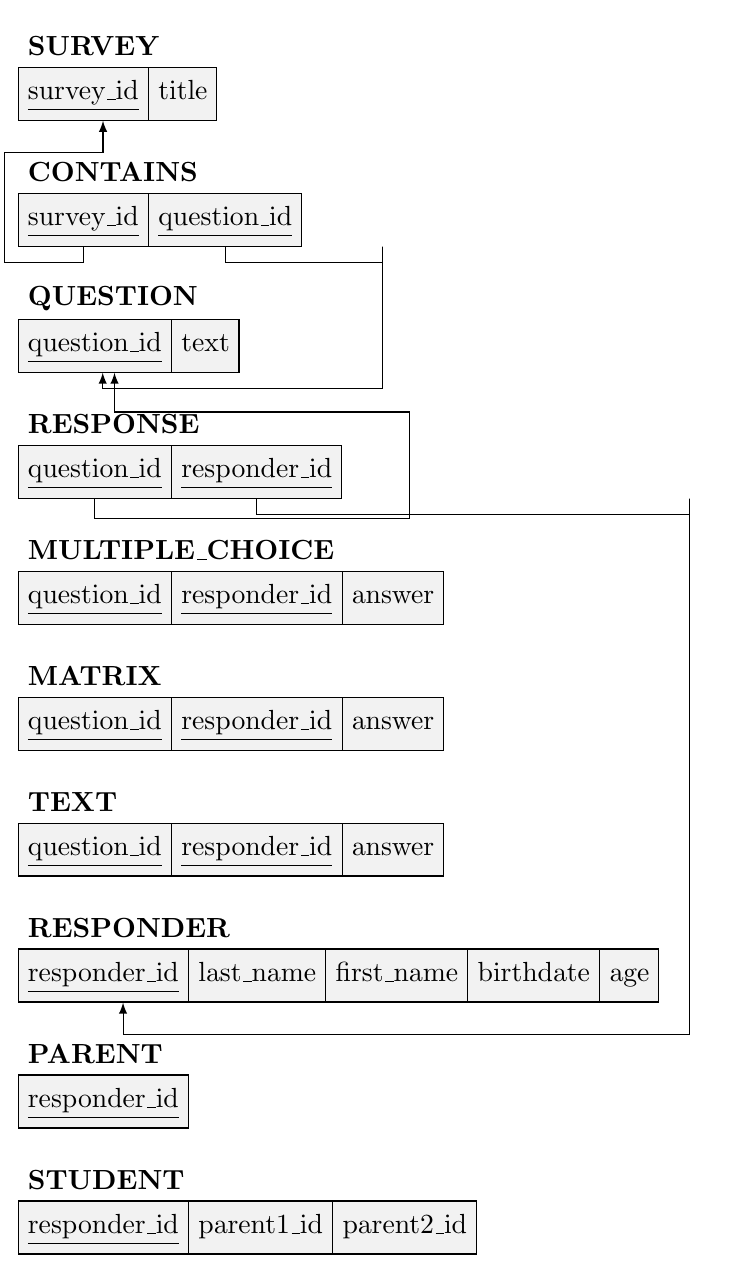
\begin{tikzpicture}[relation/.style={rectangle split, rectangle split parts=#1, rectangle split part align=base, draw, anchor=center, align=center, text height=3mm, text centered}]\hspace*{-0.3cm}

% Relations

\node (surveytitle) {\textbf{SURVEY}};
\node [relation=2, rectangle split horizontal, rectangle split part fill={lightgray!50}, anchor=north west, below=0.6cm of surveytitle.west, anchor=west] (survey)
{\underline{survey\_id}%
\nodepart{two}		title
\nodepart{three}	program};

\node [below=1cm of survey.west, anchor=west] (containstitle) {\textbf{CONTAINS}};
\node [relation=2, rectangle split horizontal, rectangle split part fill={lightgray!50}, anchor=north west, below=0.6cm of containstitle.west, anchor=west] (contains)
{\underline{survey\_id}
\nodepart{two}	\underline{question\_id}};

\node [below=1cm of contains.west, anchor=west] (questiontitle) {\textbf{QUESTION}};
\node [relation=2, rectangle split horizontal, rectangle split part fill={lightgray!50}, anchor=north west, below=0.6cm of questiontitle.west, anchor=west] (question)
{\underline{question\_id}%
\nodepart{two}		text};

\node [below=1cm of question.west, anchor=west] (responsetitle) {\textbf{RESPONSE}};
\node [relation=2, rectangle split horizontal, rectangle split part fill={lightgray!50}, anchor=north west, below=0.6cm of responsetitle.west, anchor=west] (response)
{\underline{question\_id}%
\nodepart{two}		\underline{responder\_id}};

\node [below=1cm of response.west, anchor=west] (multiplechoicetitle) {\textbf{MULTIPLE\_CHOICE}};
\node [relation=3, rectangle split horizontal, rectangle split part fill={lightgray!50}, anchor=north west, below=0.6cm of multiplechoicetitle.west, anchor=west] (multiplechoice)
{\underline{question\_id}%
\nodepart{two}		\underline{responder\_id}
\nodepart{three}	answer};

\node [below=1cm of multiplechoice.west, anchor=west] (matrixtitle) {\textbf{MATRIX}};
\node [relation=3, rectangle split horizontal, rectangle split part fill={lightgray!50}, anchor=north west, below=0.6cm of matrixtitle.west, anchor=west] (matrix)
{\underline{question\_id}%
\nodepart{two}		\underline{responder\_id}
\nodepart{three}	answer};

\node [below=1cm of matrix.west, anchor=west] (texttitle) {\textbf{TEXT}};
\node [relation=3, rectangle split horizontal, rectangle split part fill={lightgray!50}, anchor=north west, below=0.6cm of texttitle.west, anchor=west] (text)
{\underline{question\_id}%
\nodepart{two}		\underline{responder\_id}
\nodepart{three}	answer};

\node [below=1cm of text.west, anchor=west] (respondertitle) {\textbf{RESPONDER}};
\node [relation=5, rectangle split horizontal, rectangle split part fill={lightgray!50}, anchor=north west, below=0.6cm of respondertitle.west, anchor=west] (responder)
{\underline{responder\_id}%
\nodepart{two}		last\_name
\nodepart{three}	first\_name
\nodepart{four}	birthdate
\nodepart{five}		age};

\node [below=1cm of responder.west, anchor=west] (parenttitle) {\textbf{PARENT}};
\node [relation=1, rectangle split horizontal, rectangle split part fill={lightgray!50}, anchor=north west, below=0.6cm of parenttitle.west, anchor=west] (parent)
{\underline{responder\_id}};

\node [below=1cm of parent.west, anchor=west] (studenttitle) {\textbf{STUDENT}};
\node [relation=3, rectangle split horizontal, rectangle split part fill={lightgray!50}, anchor=north west, below=0.6cm of studenttitle.west, anchor=west] (student)
{\underline{responder\_id}%
\nodepart{two}		parent1\_id
\nodepart{three}	parent2\_id};

% Foreign keys

\draw[-latex] (contains.one south) -- ++(0,-0.2) -| ($(contains.one south) + (-1,0)$) |- ($(survey.one south) + (0.25,-0.40)$) -| ($(survey.one south) + (0.25,0)$);

\draw[-latex] (contains.two south) -- ++(0,-0.2) -| ($(contains.two south) + (2,0)$) |- ($(question.one south) + (0.25,-0.20)$) -| ($(question.one south) + (0.10,0)$);

\draw[-latex] (response.one south) -- ++(0,-0.25) -| ($(response.one south) + (4,0)$) |- ($(question.one south) + (0.25,-0.50)$) -| ($(question.one south) + (0.25,0)$);

\draw[-latex] (response.two south) -- ++(0,-0.2) -| ($(response.two south) + (5.50,0)$) |- ($(responder.one south) + (0.25,-0.40)$) -| ($(responder.one south) + (0.25,0)$);

\end{tikzpicture}
\captionof{figure}{The relational database schema}

\subsubsection{Database creation}
Each table will be created with the following SQL syntax.
In particular, tables will use AUTO INCREMENT to automatically increment and create IDs.
They will also be done in the following order because some tables reference others.
\lstset{language=SQL,breaklines=true,breakatwhitespace=true}
\begin{lstlisting}
CREATE TABLE Survey
(
 survey_id int NOT NULL AUTO_INCREMENT
 title varchar(255)
 program varchar(255)
 PRIMARY KEY (survey_id)
)

CREATE TABLE Question
(
 question_id int NOT NULL AUTO_INCREMENT
 text varchar(1020) NOT NULL
 PRIMARY KEY (question_id)
)

CREATE TABLE Contains
(
 survey_id int NOT NULL
 question_id int NOT NULL
 PRIMARY KEY (survey_id, question_id)
 FOREIGN KEY (survey_id) REFERENCES Survey(survey_id)
 FOREIGN KEY (question_id) REFERENCES Question(question_id)
)

CREATE TABLE Responder
(
 responder_id int NOT NULL AUTO_INCREMENT
 first_name varchar(255) NOT NULL
 last_name varchar(255) NOT NULL
 birthdate date
 age int
 PRIMARY KEY (responder_id)
)

CREATE TABLE Parent
(
 responder_id int NOT NULL
 PRIMARY KEY (responder_id)
 FOREIGN KEY (responder_id) REFERENCES Responder(responder_id)
)

CREATE TABLE Student
(
 responder_id int NOT NULL
 parent1_id int
 parent2_id int
 PRIMARY KEY (responder_id)
 FOREIGN KEY (responder_id) REFERENCES Responder(responder_id)
 FOREIGN KEY (parent1_id) REFERENCES Parent(responder_id)
 FOREIGN KEY (parent2_id) REFERENCES Parent(responder_id)
)

CREATE TABLE Response
(
 question_id int NOT NULL
 responder_id int NOT NULL
 PRIMARY KEY (question_id, responder_id)
 FOREIGN KEY (question_id) REFERENCES Question(question_id)
 FOREIGN KEY (responder_id) REFERENCES Responder(responder_id)
)

CREATE TABLE Multiple_Choice
(
 question_id int NOT NULL
 responder_id int NOT NULL
 answer char(1)
 PRIMARY KEY (question_id, responder_id)
 FOREIGN KEY (question_id) REFERENCES Question(question_id)
 FOREIGN KEY (responder_id) REFERENCES Responder(responder_id)
)

CREATE TABLE Matrix
(
 question_id int NOT NULL
 responder_id int NOT NULL
 answer int
 PRIMARY KEY (question_id, responder_id)
 FOREIGN KEY (question_id) REFERENCES Question(question_id)
 FOREIGN KEY (responder_id) REFERENCES Responder(responder_id)
)

CREATE TABLE Text
(
 question_id int NOT NULL
 responder_id int NOT NULL
 answer varchar(1020)
 PRIMARY KEY (question_id, responder_id)
 FOREIGN KEY (question_id) REFERENCES Question(question_id)
 FOREIGN KEY (responder_id) REFERENCES Responder(responder_id)
)
\end{lstlisting}

\subsubsection{Database interaction}
To allow for interaction between the survey and report generation, an API will need to be created to work with both.
The API will be written in PHP since PHP provides functionality to generate SQL queries with a database using \texttt{mysqli} objects and the \texttt{query()} function.
\subsubsection{Interacting with the survey generation}
Since the survey generation will be done using JSON, the API will need to get the POST information as the JSON object and parse it for a SQL INSERT.
It will do so using the following design:
\begin{enumerate}
	\item Generate a string \texttt{sql\_query} for the SQL query setting up the INSERT query with `INSERT INTO ` and adding the name of the table from the POST information.
	\item Because each table has different sets of attributes, a switch statement will be used to check the table name and add the necessary string to \texttt{sql\_query} (this switch statement will take the value from the POST and convert it all to lowercase).
	\begin{enumerate}
		\item The Survey table will add `(title, program)`.
		\item The Contains table will add `(survey\_id, question\_id)`.
		\item The Question table will add `(text)`.
		\item The Response table will add `(question\_id, responder\_id)`.
		\item The Multiple\_Choice, Matrix, and Text tables will add `(question\_id, responder\_id, answer)`.
		\item The Responder table will add `(last\_name, first\_name, birthdate, age)`
		\item The Student table will add `(responder\_id, parent1\_id, parent2\_id)`.
		\item The Parent table will add `(responder\_id)`.
	\end{enumerate}
	\item The string `VALUES ` will be appended to \texttt{sql\_query}.
	\item A while loop will wrap around the following process to account for multiple entries being added to the table.
	\begin{enumerate}
		\item There will be another switch structure to determine the number of values that will be inserted based on the table to be inserted into:
		\begin{enumerate}
			\item The Question, and Parent tables will read one value and add `(\emph{value1}),` to \texttt{sql\_query} accordingly.
			\item The Survey, Contains and Reponse tables will read two values and add `(\emph{value1}, \emph{value2}),` to \texttt{sql\_query}.
			\item The Multiple\_Choice, Matrix, Text, and Student tables will read three values and add `(\emph{value1}, \emph{value2}, \emph{value3}),` to \texttt{sql\_query}.
			\item The Responder table will read four values and add `(\emph{value1}, \emph{value2}, \emph{value3}, \emph{value4}, \emph{value5}),` to \texttt{sql\_query}.
		\end{enumerate}
	\end{enumerate}
	\item After the loop, the last character of \texttt{sql\_query} should be a comma, and it will be replaced with a semicolon.
	\item After the string has been completed, a mysqli object \texttt{conn} will be created that connects to the server the database is stored on.
	\item A call to \texttt{conn}'s function \texttt{query()}, passing \texttt{sql\_query} as the argument query string.
				The result will be stored in a variable called \texttt{result}.
	\item There will be a check on if the value of \texttt{result} is true.
	\begin{enumerate}
		\item If it is true, then display a success message.
		\item If it is not true, then display an error message.
	\end{enumerate}
	\item Lastly, \texttt{connection} will be closed.
\end{enumerate}

\subsubsection{Interacting with report generation}
% *** WORK IN PROGRESS ***
\begin{enumerate}
	\item The API will receive the SQL query as a string and store it as \texttt{sql\_query}.
	\item A mysqli object \texttt{conn} will be created that connects to the server the database is stored on.
	\item A call to \texttt{conn}'s function \texttt{query()}, passing \texttt{sql\_query} as the argument query string.
				The result will be stored in a variable called \texttt{result}.
	\item There will be a check on if the value of \texttt{result} is true.
	\begin{enumerate}
		\item If it is true, then display a success message.
		\item If it is not true, then display an error message.
	\end{enumerate}
	\item \texttt{connection} will be closed.
	\item Lastly, \texttt{result} will be echoed.
\end{enumerate}

\subsection{Search Form Interface}
The user interface for report generation will be a search form that uses text input boxes for querying information from the database. The fields that will be shown on the webpage include survey questions, responses, student info, club, program, and student demographic information. When the user arrives at the report generation page for the first time there will be one input text box for each field by default. Each input field will have its corresponding name written above incase the user deletes all of the input fields for the search form. This will allow the user to distinguish which add button corresponds to each field. The add button for each field will be located below the most recently created text input box. The add button will allow administrative users to add additional information for their query. Each input field will have a button on the right hand side for deleting the input field which will be indicated by "x" symbol and this will allow a user to delete any input fields that are no longer necessary for their query. Once an administrative user has finished inputting their query information into the input fields they will be able to submit their query by clicking on a submit button that will be located on the bottom right hand side of the search form. Below the search form there will an empty report form if the user decided to create a new report. If the user decided to edit a saved report the report form will display the query results of their saved report. 

\subsubsection{Search Form Logic} 
 For creating the report generation form we will be using AngularJS, HTML, and PHP. The reason for using AngularJS is that it will enable us to create a dynamic search form which will allow the user to add additional input fields for their query. If we did not use AngularJS the form would be static and if an administrative user were to need more input fields for their query they would have to notify a developer to add the input fields manually to the HTML page which is inefficient. AngularJS requires an HTML for defining the application's user interface \cite{Lau}. The buttons for deleting and adding new input fields will have an ng-click AngularJS directive which will call their correspoding function for deleting and adding a new input field.  A controller will be used to modify the HTML expressions and the \$scope service will be used to detect any changes in the form\cite{Rav}.

\subsubsection{Report Generation Interface} 
When an administrative user has finished querying information for their report form they will be able to save their report by clicking on a save button that will be located at the bottom right hand side of the report form.Administrative users will be able to print out their generated reports or any saved reports by clicking on a print button that will be located on the top right hand side on the report form.


\subsubsection{Report Generation Logic}
 In order to save the report a table will be created in the database that only stores reports. By creating a table for storing reports it will permanently save them unless they are deleted from the database. PHP will be used for saving reports into the database and this will be done by using the INSERT INTO statement. For printing the report form CSS and Javascript will be used. CSS will be used to create two style sheets, so that when the print button is clicked it does not display the entire webpage as the content that is going to be printed. The first style sheet will be used to display the contents of the report generation webpage. The second style sheet will be used to exclude content on the webpage that is not related to the search form. For displaying the print dialogue box the line of code href="javascript:window.print()" will be added to the print button. The print dialogue box will allow adminstrative users to choose the orientation, number of copies to be printed, margins, page range, etc. When the submit button is clicked PHP will be used to query the information from the database using the SELECT statement. Any input text box fields left empty will be ignored when the submit button is clicked. The results of the query will be inserted into an empty form that will be located below the search form for making queries. The form will be created using the HTML $<$form$>$ tag and each query result will be saved into a $<$input$>$ element that has the type text. 

The report form will be saved as a json object. The structure that the report form will have is the following:\\
\{ \\
	\indent id: random numerical value to identify the report\\
	\indent title: string that contains the title of the report\\
	\indent queries: an array of queries contained in the report \\
\} 

The queries made by administrative users will be saved as json objects. The following is the structure of the queries:\\
\{\\
	\indent id: a unique identifier for each query\\
	\indent result: the text result of the query generated by an administrative user\\
\}\\

%\subsection{Design viewpoint \emph{i}}
%\subsection{Design view \emph{i}}
%\subsection{Design rationale}


\end{document}
